\chapter{Evaluación}
\label{chap:evaluation}
\vspace{0.5cm}

%%%%%%%%%%%%%%%%%%%%%%%%%%%%%%%%%%%%%%%%%%%%%%%%%%%%%%%%%%%%%%%%%%%%%%%%%%%%%%%%
% Objetivo: Exponer los resultados objetivos del sistema                       %
%%%%%%%%%%%%%%%%%%%%%%%%%%%%%%%%%%%%%%%%%%%%%%%%%%%%%%%%%%%%%%%%%%%%%%%%%%%%%%%%

 \lettrine{E}{n} este capítulo exponen los resultados de la evaluación del sistema. Se han seleccionado tres piezas musicales conocidas para realizar las diferentes pruebas. A continuación se describen las tres piezas y las pruebas realizadas. Para realizar una prueba de carga que establezca los límites del sistema se ha añadido una última partitura suficientemente sencilla sobre la que trabajar para poder realizar estas pruebas cómodamente sin preocuparse por la calidad de los resultados.
 
 \begin{itemize}
 	\item \textbf{Menuet:} Famosa pieza de Johann S. Bach, destaca por su simpleza y es interesante para ver como funciona el programa ante compases ternarios. Se sugiere añadir una voz nueva de tesitura más aguda a la presente en la pieza.
 	\item \textbf{Greensleves:} Supuestamente compuesta por Enrique VIII, esta archiconocida partitura presenta una polifonía coral a cuatro voces, ideal para comprobar las capacidades de armonización del sistema. Se sugiere eliminar secciones grandes de la voz solista y ver cómo la completa.
 	\item \textbf{Joy to the World:} Conocido villancico, sería interesante escuchar una reinterpretación de la voz más grave para la pieza, ya sea completando secciones o bien añadiendo una voz de bajo.
 	\item \textbf{The Legend of Zelda:} Tema principal de la conocida saga de videojuegos con el mismo nombre, se ha buscado un arreglo muy sencillo y cercano a la pieza original en 8-bit para poder realizar las pruebas de carga sobre esta pieza.
 \end{itemize}
 
 Para la evaluación se han realizado armonizaciones de todas las piezas y se han medido los tiempos y la calidad de las mismas, además se han realizado pruebas de completado de un compás en cada pieza junto con la inclusión de una nueva voz, también se han medido calidad y tiempo. Por último, con la partitura de \textit{The Legend of Zelda} se han realizado pruebas para comprobar hasta donde funciona bien en cuestión temporal, para ello se ha ido vaciando porcentualmente una de las voces para ser completada y después se han ido añadiendo diferentes voces.
 
 Nótese que debido al carácter no-determinista de \textit{Answer Set Programming} y a los tiempos de entrada y salida estos tiempos sirven para dar una idea aproximada de los tiempos de funcionamiento de la herramienta. Para suavizar los valores dispares se ha ejecutado cada medida 100 veces, se ha restado el tiempo de usuario y se ha calculado el tiempo promedio. 
 
 \begin{figure}
 	\centering
 	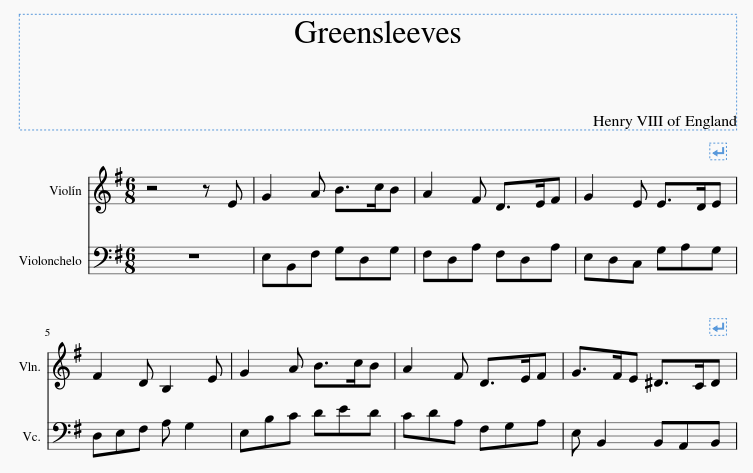
\includegraphics[width=0.8\linewidth]{imagenes/evaluation/greensleeves_orig.png}
 	\caption{Comienzo de Greensleeves sin armonizar}
 	\label{fig:greensleeves_orig}
 \end{figure}
 
  \begin{figure}
  	\centering
  	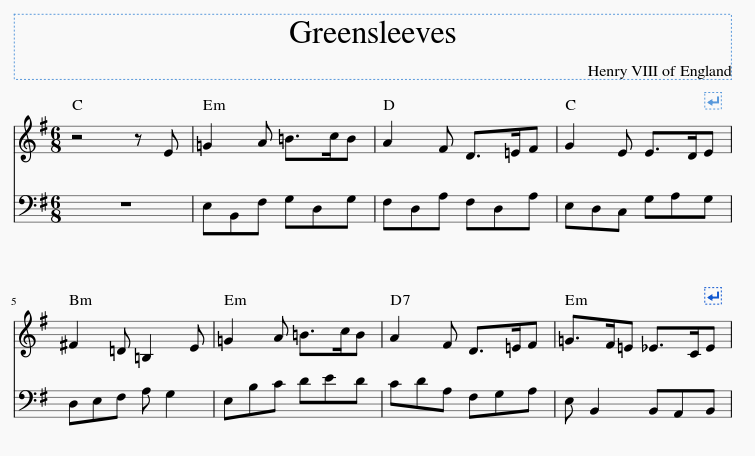
\includegraphics[width=0.8\linewidth]{imagenes/evaluation/greensleeves_harm.png}
  	\caption{Comienzo de Greensleeves armonizado}
  	\label{fig:greensleeves_harm}
  \end{figure}
  
   \begin{figure}
   	\centering
   	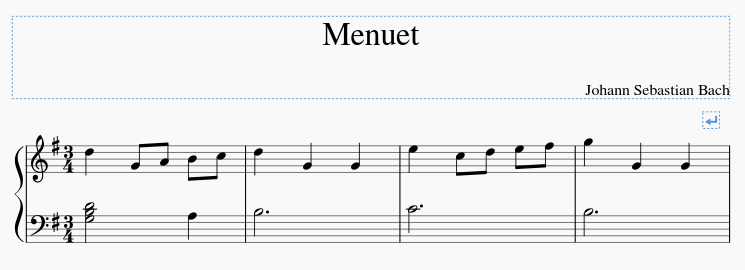
\includegraphics[width=0.8\linewidth]{imagenes/evaluation/menuet_orig.png}
   	\caption{Comienzo de Menuet sin armonizar}
   	\label{fig:menuet_orig}
   \end{figure}
   
    \begin{figure}
    	\centering
    	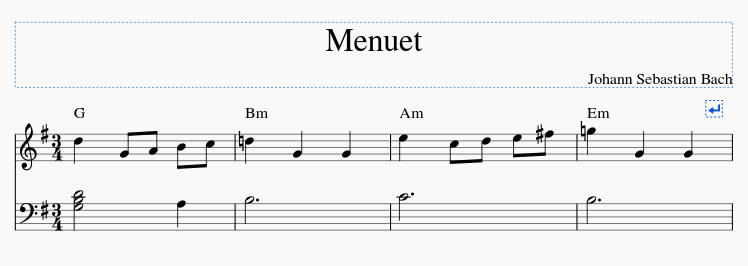
\includegraphics[width=0.8\linewidth]{imagenes/evaluation/menuet_harm.png}
    	\caption{Comienzo de Menuet armonizado}
    	\label{fig:menuet_harm}
    \end{figure}
     \begin{figure}
     	\centering
     	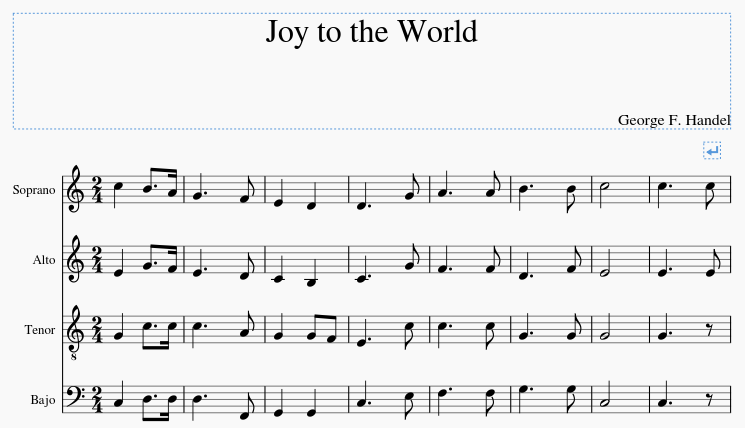
\includegraphics[width=0.8\linewidth]{imagenes/evaluation/joy_orig.png}
     	\caption{Comienzo de Joy to the World sin armonizar}
     	\label{fig:joy_orig}
     \end{figure}
  
        \begin{figure}
        	\centering
        	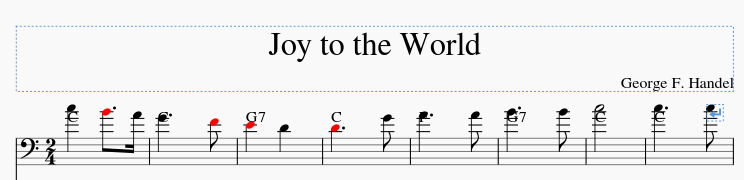
\includegraphics[width=0.8\linewidth]{imagenes/evaluation/joy_harm_err.png}
        	\caption{La salida de Joy to the World produce un error de clave en la voz de la Soprano}
        	\label{fig:joy_harm_err}
        \end{figure}
     
      \begin{figure}
      	\centering
      	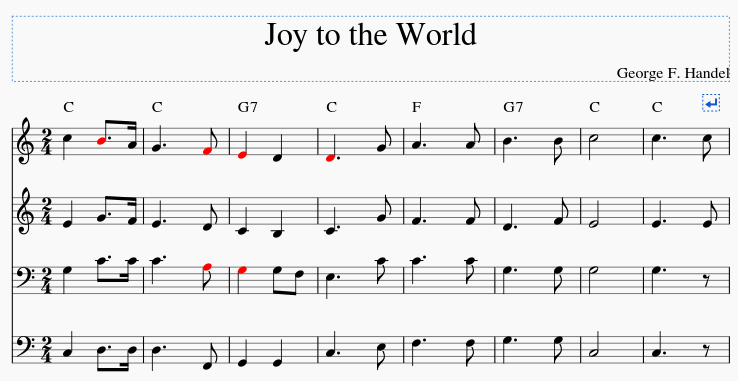
\includegraphics[width=0.8\linewidth]{imagenes/evaluation/joy_harm.png}
      	\caption{Comienzo de Joy to the World armonizado}
      	\label{fig:joy_harm}
      \end{figure}
  
  \begin{center}
  	\begin{tabular}{ | l | c | c | c | }
  		\hline
  		Pieza & T. Armonización & T. Compás & T. Nueva voz \\ \hline \hline
  		Greensleeves & 0.5922s & 0 & 0 \\ \hline
  		Menuet & 0.912s & 0 & 0 \\ \hline
  		Joy to the World & 4.378s & 0 & 0 \\ \hline
  		The Legend of Zelda & 0s & 0 & 0 \\ \hline
  	\end{tabular}
  \end{center}
  
  

